\section{Volume averaging}

\begin{frame}{Representative Elementary Volume}

    \begin{figure}
        \centering
        \includesvg[width=0.6\linewidth]{media/profile_porous_V.svg}
    \end{figure}

    $$\varrho\frac{\partial u}{\partial t} + \varrho (u\cdot\nabla)u = \varrho g - \nabla p + \nabla\cdot(\tau_v+\tau_t)\ ,\quad {\color{toravalr}u \leftarrow \frac{1}{V~}\int_{\mathcal V} u ~\mathrm dV}$$

    $$\varrho\frac{\partial u}{\partial t} + \varrho (u\cdot\nabla)u = \varrho g - \nabla p + \nabla\cdot(\tau_v+\tau_t+{\color{toravalr}\tau_d}) + {\color{toravalr}\epsilon f} - {\color{toravalr}\mu\nabla u\nabla\epsilon}$$

    % $$\Rightarrow \begin{cases}
    %     \text{Additional stresses in momentum balance :}~\tau_t+\tau_d\\
    %     \text{Drag force density (Darcy) naturally appears :}~f
    % \end{cases}$$

    \bigskip

    \anonymousfootnote{\cite{vlad}}
\end{frame}

\begin{frame}{Steady-state uniform flow equation}{A single ODE}

    \begin{columns}
        \column{0.66\linewidth}
            \begin{figure}
                \centering
                \includesvg[width=\linewidth]{media/profile_porous_V_smoothed.svg}
            \end{figure}
        
        \column{0.33\linewidth}
        \begin{figure}
            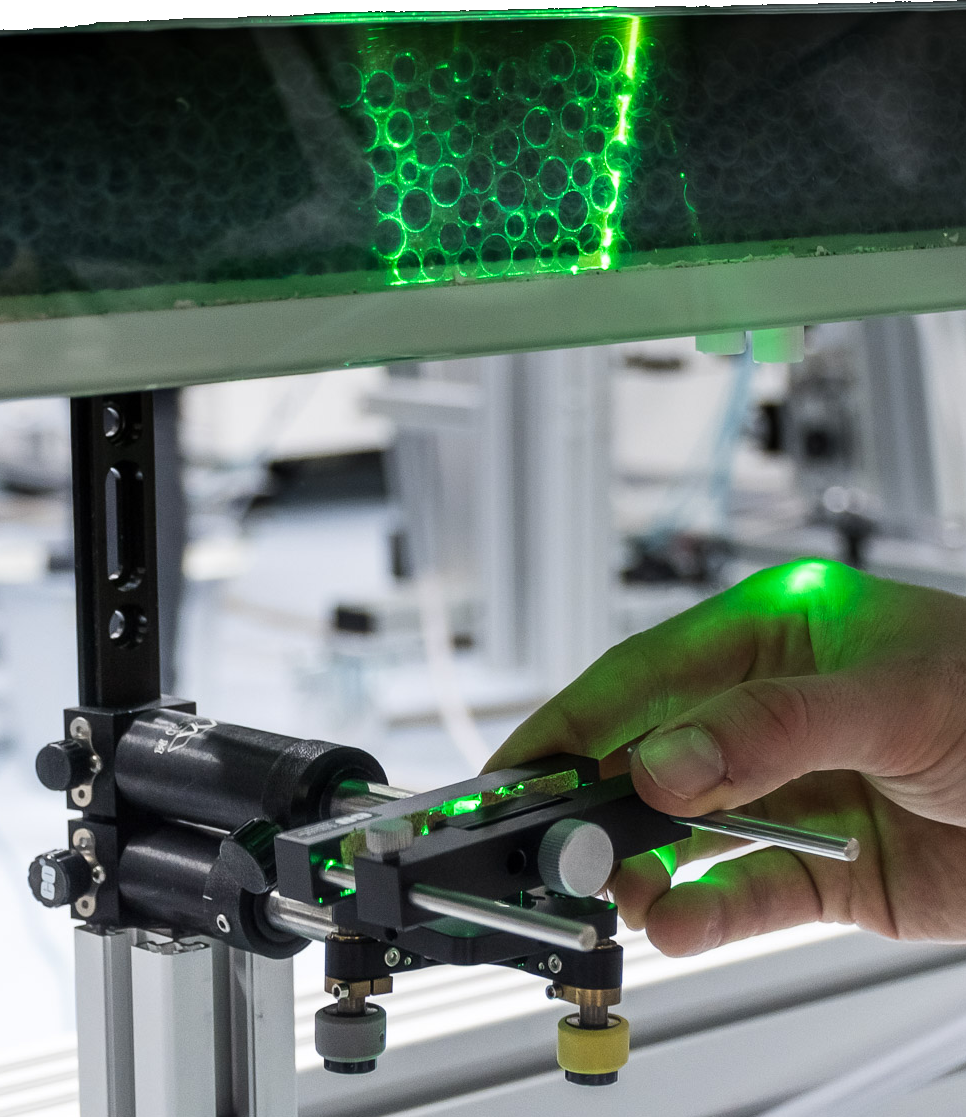
\includegraphics[width=\linewidth]{media/PIV-RIMS_cropped.png}
        \end{figure}
        
    \end{columns}

    \bigskip

    $$0 = \epsilon \varrho g i + \frac{\mathrm d(\tau_v + \tau_t + \tau_d)}{\mathrm dz} + \epsilon f - \mu \frac{\mathrm d u}{\mathrm dz}\frac{\mathrm d\epsilon}{\mathrm dz}$$

    \anonymousfootnote{\cite{Rousseau_Ancey_2022}}
\end{frame}

